\documentclass[twoside]{book}

% Packages required by doxygen
\usepackage{fixltx2e}
\usepackage{calc}
\usepackage{doxygen}
\usepackage[export]{adjustbox} % also loads graphicx
\usepackage{graphicx}
\usepackage[utf8]{inputenc}
\usepackage{makeidx}
\usepackage{multicol}
\usepackage{multirow}
\PassOptionsToPackage{warn}{textcomp}
\usepackage{textcomp}
\usepackage[nointegrals]{wasysym}
\usepackage[table]{xcolor}

% Font selection
\usepackage[T1]{fontenc}
\usepackage[scaled=.90]{helvet}
\usepackage{courier}
\usepackage{amssymb}
\usepackage{sectsty}
\renewcommand{\familydefault}{\sfdefault}
\allsectionsfont{%
  \fontseries{bc}\selectfont%
  \color{darkgray}%
}
\renewcommand{\DoxyLabelFont}{%
  \fontseries{bc}\selectfont%
  \color{darkgray}%
}
\newcommand{\+}{\discretionary{\mbox{\scriptsize$\hookleftarrow$}}{}{}}

% Page & text layout
\usepackage{geometry}
\geometry{%
  a4paper,%
  top=2.5cm,%
  bottom=2.5cm,%
  left=2.5cm,%
  right=2.5cm%
}
\tolerance=750
\hfuzz=15pt
\hbadness=750
\setlength{\emergencystretch}{15pt}
\setlength{\parindent}{0cm}
\setlength{\parskip}{3ex plus 2ex minus 2ex}
\makeatletter
\renewcommand{\paragraph}{%
  \@startsection{paragraph}{4}{0ex}{-1.0ex}{1.0ex}{%
    \normalfont\normalsize\bfseries\SS@parafont%
  }%
}
\renewcommand{\subparagraph}{%
  \@startsection{subparagraph}{5}{0ex}{-1.0ex}{1.0ex}{%
    \normalfont\normalsize\bfseries\SS@subparafont%
  }%
}
\makeatother

% Headers & footers
\usepackage{fancyhdr}
\pagestyle{fancyplain}
\fancyhead[LE]{\fancyplain{}{\bfseries\thepage}}
\fancyhead[CE]{\fancyplain{}{}}
\fancyhead[RE]{\fancyplain{}{\bfseries\leftmark}}
\fancyhead[LO]{\fancyplain{}{\bfseries\rightmark}}
\fancyhead[CO]{\fancyplain{}{}}
\fancyhead[RO]{\fancyplain{}{\bfseries\thepage}}
\fancyfoot[LE]{\fancyplain{}{}}
\fancyfoot[CE]{\fancyplain{}{}}
\fancyfoot[RE]{\fancyplain{}{\bfseries\scriptsize Generated by Doxygen }}
\fancyfoot[LO]{\fancyplain{}{\bfseries\scriptsize Generated by Doxygen }}
\fancyfoot[CO]{\fancyplain{}{}}
\fancyfoot[RO]{\fancyplain{}{}}
\renewcommand{\footrulewidth}{0.4pt}
\renewcommand{\chaptermark}[1]{%
  \markboth{#1}{}%
}
\renewcommand{\sectionmark}[1]{%
  \markright{\thesection\ #1}%
}

% Indices & bibliography
\usepackage{natbib}
\usepackage[titles]{tocloft}
\setcounter{tocdepth}{3}
\setcounter{secnumdepth}{5}
\makeindex

% Hyperlinks (required, but should be loaded last)
\usepackage{ifpdf}
\ifpdf
  \usepackage[pdftex,pagebackref=true]{hyperref}
\else
  \usepackage[ps2pdf,pagebackref=true]{hyperref}
\fi
\hypersetup{%
  colorlinks=true,%
  linkcolor=blue,%
  citecolor=blue,%
  unicode%
}

% Custom commands
\newcommand{\clearemptydoublepage}{%
  \newpage{\pagestyle{empty}\cleardoublepage}%
}

\usepackage{caption}
\captionsetup{labelsep=space,justification=centering,font={bf},singlelinecheck=off,skip=4pt,position=top}

%===== C O N T E N T S =====

\begin{document}

% Titlepage & ToC
\hypersetup{pageanchor=false,
             bookmarksnumbered=true,
             pdfencoding=unicode
            }
\pagenumbering{roman}
\begin{titlepage}
\vspace*{7cm}
\begin{center}%
{\Large My Project }\\
\vspace*{1cm}
{\large Generated by Doxygen 1.8.11}\\
\end{center}
\end{titlepage}
\clearemptydoublepage
\tableofcontents
\clearemptydoublepage
\pagenumbering{arabic}
\hypersetup{pageanchor=true}

%--- Begin generated contents ---
\chapter{Namespace Index}
\section{Namespace List}
Here is a list of all namespaces with brief descriptions\+:\begin{DoxyCompactList}
\item\contentsline{section}{\hyperlink{namespacequeuesavitch}{queuesavitch} }{\pageref{namespacequeuesavitch}}{}
\end{DoxyCompactList}

\chapter{File Index}
\section{File List}
Here is a list of all files with brief descriptions\+:\begin{DoxyCompactList}
\item\contentsline{section}{\hyperlink{Lab1_8c}{Lab1.\+c} }{\pageref{Lab1_8c}}{}
\end{DoxyCompactList}

\chapter{Namespace Documentation}
\hypertarget{namespaceaddAccount}{}\section{add\+Account Namespace Reference}
\label{namespaceaddAccount}\index{add\+Account@{add\+Account}}
\subsection*{Functions}
\begin{DoxyCompactItemize}
\item 
def \hyperlink{namespaceaddAccount_a3a8c94acd800e708964781259da98d47}{get\+Information} ()
\item 
def \hyperlink{namespaceaddAccount_ada25390ce86fe3bb69a36068bfb536e2}{create\+Account} (i, p)
\item 
def \hyperlink{namespaceaddAccount_adae774fe357f7b01357de9919b9e9da5}{set\+P\+IN} ()
\end{DoxyCompactItemize}
\subsection*{Variables}
\begin{DoxyCompactItemize}
\item 
\hyperlink{namespaceaddAccount_a54cf092e8aeaae1cd4b3d502f239ae08}{information} = \hyperlink{namespaceaddAccount_a3a8c94acd800e708964781259da98d47}{get\+Information}()
\item 
\hyperlink{namespaceaddAccount_ae10ea4b40c1517c05f038e86e63fb541}{pin} = \hyperlink{namespaceaddAccount_adae774fe357f7b01357de9919b9e9da5}{set\+P\+IN}()
\end{DoxyCompactItemize}


\subsection{Function Documentation}
\index{add\+Account@{add\+Account}!create\+Account@{create\+Account}}
\index{create\+Account@{create\+Account}!add\+Account@{add\+Account}}
\subsubsection[{\texorpdfstring{create\+Account(i, p)}{createAccount(i, p)}}]{\setlength{\rightskip}{0pt plus 5cm}def add\+Account.\+create\+Account (
\begin{DoxyParamCaption}
\item[{}]{i, }
\item[{}]{p}
\end{DoxyParamCaption}
)}\hypertarget{namespaceaddAccount_ada25390ce86fe3bb69a36068bfb536e2}{}\label{namespaceaddAccount_ada25390ce86fe3bb69a36068bfb536e2}


Here is the call graph for this function\+:
\nopagebreak
\begin{figure}[H]
\begin{center}
\leavevmode
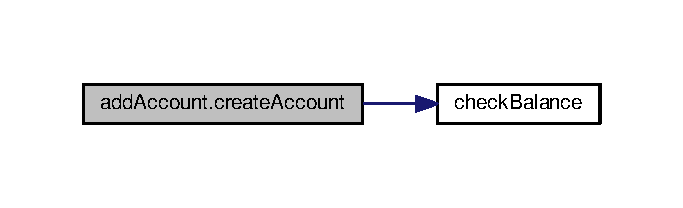
\includegraphics[width=328pt]{namespaceaddAccount_ada25390ce86fe3bb69a36068bfb536e2_cgraph}
\end{center}
\end{figure}


\index{add\+Account@{add\+Account}!get\+Information@{get\+Information}}
\index{get\+Information@{get\+Information}!add\+Account@{add\+Account}}
\subsubsection[{\texorpdfstring{get\+Information()}{getInformation()}}]{\setlength{\rightskip}{0pt plus 5cm}def add\+Account.\+get\+Information (
\begin{DoxyParamCaption}
{}
\end{DoxyParamCaption}
)}\hypertarget{namespaceaddAccount_a3a8c94acd800e708964781259da98d47}{}\label{namespaceaddAccount_a3a8c94acd800e708964781259da98d47}
\index{add\+Account@{add\+Account}!set\+P\+IN@{set\+P\+IN}}
\index{set\+P\+IN@{set\+P\+IN}!add\+Account@{add\+Account}}
\subsubsection[{\texorpdfstring{set\+P\+I\+N()}{setPIN()}}]{\setlength{\rightskip}{0pt plus 5cm}def add\+Account.\+set\+P\+IN (
\begin{DoxyParamCaption}
{}
\end{DoxyParamCaption}
)}\hypertarget{namespaceaddAccount_adae774fe357f7b01357de9919b9e9da5}{}\label{namespaceaddAccount_adae774fe357f7b01357de9919b9e9da5}


Here is the call graph for this function\+:
\nopagebreak
\begin{figure}[H]
\begin{center}
\leavevmode
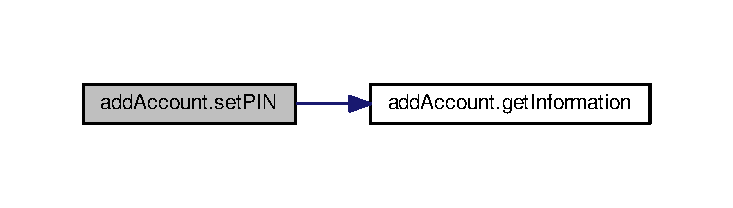
\includegraphics[width=350pt]{namespaceaddAccount_adae774fe357f7b01357de9919b9e9da5_cgraph}
\end{center}
\end{figure}




\subsection{Variable Documentation}
\index{add\+Account@{add\+Account}!information@{information}}
\index{information@{information}!add\+Account@{add\+Account}}
\subsubsection[{\texorpdfstring{information}{information}}]{\setlength{\rightskip}{0pt plus 5cm}add\+Account.\+information = {\bf get\+Information}()}\hypertarget{namespaceaddAccount_a54cf092e8aeaae1cd4b3d502f239ae08}{}\label{namespaceaddAccount_a54cf092e8aeaae1cd4b3d502f239ae08}
\index{add\+Account@{add\+Account}!pin@{pin}}
\index{pin@{pin}!add\+Account@{add\+Account}}
\subsubsection[{\texorpdfstring{pin}{pin}}]{\setlength{\rightskip}{0pt plus 5cm}add\+Account.\+pin = {\bf set\+P\+IN}()}\hypertarget{namespaceaddAccount_ae10ea4b40c1517c05f038e86e63fb541}{}\label{namespaceaddAccount_ae10ea4b40c1517c05f038e86e63fb541}

\hypertarget{namespaceBalance}{}\section{Balance Namespace Reference}
\label{namespaceBalance}\index{Balance@{Balance}}
\subsection*{Functions}
\begin{DoxyCompactItemize}
\item 
def \hyperlink{namespaceBalance_a0d3d5e4b10843823c119cb200c8eea1a}{get\+Account\+Number} ()
\item 
def \hyperlink{namespaceBalance_add692cc47f5beab77cc3eded4397ee84}{get\+P\+IN} (n)
\item 
def \hyperlink{namespaceBalance_a2087471cfcf15c70932c7a400f6e8b00}{find\+Balance} (a, n)
\item 
def \hyperlink{namespaceBalance_afedee86fdf9a70c8269974c695523986}{print\+Balace} (b)
\end{DoxyCompactItemize}
\subsection*{Variables}
\begin{DoxyCompactItemize}
\item 
\hyperlink{namespaceBalance_a526eb4cc966158b4a4d3b8d33c04340f}{account\+Number} = \hyperlink{namespaceBalance_a0d3d5e4b10843823c119cb200c8eea1a}{get\+Account\+Number}()
\item 
\hyperlink{namespaceBalance_a4cfe14f6e735fe18092e9809e4886137}{pin} = \hyperlink{namespaceBalance_add692cc47f5beab77cc3eded4397ee84}{get\+P\+IN}(\hyperlink{namespaceBalance_a526eb4cc966158b4a4d3b8d33c04340f}{account\+Number})
\item 
\hyperlink{namespaceBalance_a3a307687cae8694689c16220a9bb081c}{balance} = \hyperlink{namespaceBalance_a2087471cfcf15c70932c7a400f6e8b00}{find\+Balance}(\hyperlink{namespaceBalance_a526eb4cc966158b4a4d3b8d33c04340f}{account\+Number}, \hyperlink{namespaceBalance_a4cfe14f6e735fe18092e9809e4886137}{pin})
\end{DoxyCompactItemize}


\subsection{Function Documentation}
\index{Balance@{Balance}!find\+Balance@{find\+Balance}}
\index{find\+Balance@{find\+Balance}!Balance@{Balance}}
\subsubsection[{\texorpdfstring{find\+Balance(a, n)}{findBalance(a, n)}}]{\setlength{\rightskip}{0pt plus 5cm}def Balance.\+find\+Balance (
\begin{DoxyParamCaption}
\item[{}]{a, }
\item[{}]{n}
\end{DoxyParamCaption}
)}\hypertarget{namespaceBalance_a2087471cfcf15c70932c7a400f6e8b00}{}\label{namespaceBalance_a2087471cfcf15c70932c7a400f6e8b00}
\index{Balance@{Balance}!get\+Account\+Number@{get\+Account\+Number}}
\index{get\+Account\+Number@{get\+Account\+Number}!Balance@{Balance}}
\subsubsection[{\texorpdfstring{get\+Account\+Number()}{getAccountNumber()}}]{\setlength{\rightskip}{0pt plus 5cm}def Balance.\+get\+Account\+Number (
\begin{DoxyParamCaption}
{}
\end{DoxyParamCaption}
)}\hypertarget{namespaceBalance_a0d3d5e4b10843823c119cb200c8eea1a}{}\label{namespaceBalance_a0d3d5e4b10843823c119cb200c8eea1a}
\index{Balance@{Balance}!get\+P\+IN@{get\+P\+IN}}
\index{get\+P\+IN@{get\+P\+IN}!Balance@{Balance}}
\subsubsection[{\texorpdfstring{get\+P\+I\+N(n)}{getPIN(n)}}]{\setlength{\rightskip}{0pt plus 5cm}def Balance.\+get\+P\+IN (
\begin{DoxyParamCaption}
\item[{}]{n}
\end{DoxyParamCaption}
)}\hypertarget{namespaceBalance_add692cc47f5beab77cc3eded4397ee84}{}\label{namespaceBalance_add692cc47f5beab77cc3eded4397ee84}
\index{Balance@{Balance}!print\+Balace@{print\+Balace}}
\index{print\+Balace@{print\+Balace}!Balance@{Balance}}
\subsubsection[{\texorpdfstring{print\+Balace(b)}{printBalace(b)}}]{\setlength{\rightskip}{0pt plus 5cm}def Balance.\+print\+Balace (
\begin{DoxyParamCaption}
\item[{}]{b}
\end{DoxyParamCaption}
)}\hypertarget{namespaceBalance_afedee86fdf9a70c8269974c695523986}{}\label{namespaceBalance_afedee86fdf9a70c8269974c695523986}


\subsection{Variable Documentation}
\index{Balance@{Balance}!account\+Number@{account\+Number}}
\index{account\+Number@{account\+Number}!Balance@{Balance}}
\subsubsection[{\texorpdfstring{account\+Number}{accountNumber}}]{\setlength{\rightskip}{0pt plus 5cm}Balance.\+account\+Number = {\bf get\+Account\+Number}()}\hypertarget{namespaceBalance_a526eb4cc966158b4a4d3b8d33c04340f}{}\label{namespaceBalance_a526eb4cc966158b4a4d3b8d33c04340f}
\index{Balance@{Balance}!balance@{balance}}
\index{balance@{balance}!Balance@{Balance}}
\subsubsection[{\texorpdfstring{balance}{balance}}]{\setlength{\rightskip}{0pt plus 5cm}Balance.\+balance = {\bf find\+Balance}({\bf account\+Number}, {\bf pin})}\hypertarget{namespaceBalance_a3a307687cae8694689c16220a9bb081c}{}\label{namespaceBalance_a3a307687cae8694689c16220a9bb081c}
\index{Balance@{Balance}!pin@{pin}}
\index{pin@{pin}!Balance@{Balance}}
\subsubsection[{\texorpdfstring{pin}{pin}}]{\setlength{\rightskip}{0pt plus 5cm}Balance.\+pin = {\bf get\+P\+IN}({\bf account\+Number})}\hypertarget{namespaceBalance_a4cfe14f6e735fe18092e9809e4886137}{}\label{namespaceBalance_a4cfe14f6e735fe18092e9809e4886137}

\hypertarget{namespaceDeposit}{}\section{Deposit Namespace Reference}
\label{namespaceDeposit}\index{Deposit@{Deposit}}
\subsection*{Functions}
\begin{DoxyCompactItemize}
\item 
def \hyperlink{namespaceDeposit_a5550db47d340cfbf8da0504fdbb4bd38}{get\+Account\+Number} ()
\item 
def \hyperlink{namespaceDeposit_aeb2bde95c577d37691610d458bba8d96}{get\+P\+IN} (n)
\item 
def \hyperlink{namespaceDeposit_a1980b46e5ca4ad7fe16e06703b568f78}{get\+Amount} ()
\item 
def \hyperlink{namespaceDeposit_ae5cbbb64bef92d28ac3283006f0ac72c}{take\+Picture\+Of\+Check} ()
\item 
def \hyperlink{namespaceDeposit_ae9c9febfed3a8d6ad618d2c123df4b77}{deposit\+Check} (n, p, a)
\item 
def \hyperlink{namespaceDeposit_a7d4afe0289e672f39e4951c790cf8927}{print\+Confirmation} ()
\end{DoxyCompactItemize}
\subsection*{Variables}
\begin{DoxyCompactItemize}
\item 
\hyperlink{namespaceDeposit_a266a490bcb8b7e116e4e7258429aabe5}{account\+Number} = \hyperlink{namespaceDeposit_a5550db47d340cfbf8da0504fdbb4bd38}{get\+Account\+Number}()
\item 
\hyperlink{namespaceDeposit_a5ae26ec6c68e4031fbb50c9b0b15daf7}{pin} = \hyperlink{namespaceDeposit_aeb2bde95c577d37691610d458bba8d96}{get\+P\+IN}()
\item 
\hyperlink{namespaceDeposit_a903d2b091ff78ff14bb2e0e6b002de77}{amount} = \hyperlink{namespaceDeposit_a1980b46e5ca4ad7fe16e06703b568f78}{get\+Amount}()
\end{DoxyCompactItemize}


\subsection{Function Documentation}
\index{Deposit@{Deposit}!deposit\+Check@{deposit\+Check}}
\index{deposit\+Check@{deposit\+Check}!Deposit@{Deposit}}
\subsubsection[{\texorpdfstring{deposit\+Check(n, p, a)}{depositCheck(n, p, a)}}]{\setlength{\rightskip}{0pt plus 5cm}def Deposit.\+deposit\+Check (
\begin{DoxyParamCaption}
\item[{}]{n, }
\item[{}]{p, }
\item[{}]{a}
\end{DoxyParamCaption}
)}\hypertarget{namespaceDeposit_ae9c9febfed3a8d6ad618d2c123df4b77}{}\label{namespaceDeposit_ae9c9febfed3a8d6ad618d2c123df4b77}


Here is the call graph for this function\+:
\nopagebreak
\begin{figure}[H]
\begin{center}
\leavevmode
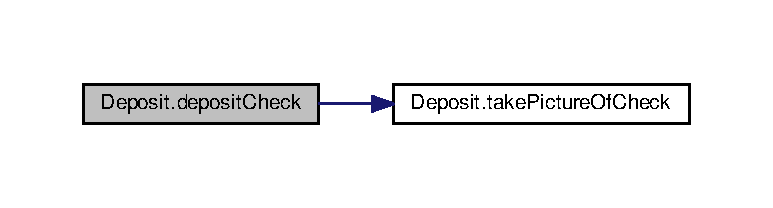
\includegraphics[width=350pt]{namespaceDeposit_ae9c9febfed3a8d6ad618d2c123df4b77_cgraph}
\end{center}
\end{figure}


\index{Deposit@{Deposit}!get\+Account\+Number@{get\+Account\+Number}}
\index{get\+Account\+Number@{get\+Account\+Number}!Deposit@{Deposit}}
\subsubsection[{\texorpdfstring{get\+Account\+Number()}{getAccountNumber()}}]{\setlength{\rightskip}{0pt plus 5cm}def Deposit.\+get\+Account\+Number (
\begin{DoxyParamCaption}
{}
\end{DoxyParamCaption}
)}\hypertarget{namespaceDeposit_a5550db47d340cfbf8da0504fdbb4bd38}{}\label{namespaceDeposit_a5550db47d340cfbf8da0504fdbb4bd38}
\index{Deposit@{Deposit}!get\+Amount@{get\+Amount}}
\index{get\+Amount@{get\+Amount}!Deposit@{Deposit}}
\subsubsection[{\texorpdfstring{get\+Amount()}{getAmount()}}]{\setlength{\rightskip}{0pt plus 5cm}def Deposit.\+get\+Amount (
\begin{DoxyParamCaption}
{}
\end{DoxyParamCaption}
)}\hypertarget{namespaceDeposit_a1980b46e5ca4ad7fe16e06703b568f78}{}\label{namespaceDeposit_a1980b46e5ca4ad7fe16e06703b568f78}
\index{Deposit@{Deposit}!get\+P\+IN@{get\+P\+IN}}
\index{get\+P\+IN@{get\+P\+IN}!Deposit@{Deposit}}
\subsubsection[{\texorpdfstring{get\+P\+I\+N(n)}{getPIN(n)}}]{\setlength{\rightskip}{0pt plus 5cm}def Deposit.\+get\+P\+IN (
\begin{DoxyParamCaption}
\item[{}]{n}
\end{DoxyParamCaption}
)}\hypertarget{namespaceDeposit_aeb2bde95c577d37691610d458bba8d96}{}\label{namespaceDeposit_aeb2bde95c577d37691610d458bba8d96}
\index{Deposit@{Deposit}!print\+Confirmation@{print\+Confirmation}}
\index{print\+Confirmation@{print\+Confirmation}!Deposit@{Deposit}}
\subsubsection[{\texorpdfstring{print\+Confirmation()}{printConfirmation()}}]{\setlength{\rightskip}{0pt plus 5cm}def Deposit.\+print\+Confirmation (
\begin{DoxyParamCaption}
{}
\end{DoxyParamCaption}
)}\hypertarget{namespaceDeposit_a7d4afe0289e672f39e4951c790cf8927}{}\label{namespaceDeposit_a7d4afe0289e672f39e4951c790cf8927}
\index{Deposit@{Deposit}!take\+Picture\+Of\+Check@{take\+Picture\+Of\+Check}}
\index{take\+Picture\+Of\+Check@{take\+Picture\+Of\+Check}!Deposit@{Deposit}}
\subsubsection[{\texorpdfstring{take\+Picture\+Of\+Check()}{takePictureOfCheck()}}]{\setlength{\rightskip}{0pt plus 5cm}def Deposit.\+take\+Picture\+Of\+Check (
\begin{DoxyParamCaption}
{}
\end{DoxyParamCaption}
)}\hypertarget{namespaceDeposit_ae5cbbb64bef92d28ac3283006f0ac72c}{}\label{namespaceDeposit_ae5cbbb64bef92d28ac3283006f0ac72c}


\subsection{Variable Documentation}
\index{Deposit@{Deposit}!account\+Number@{account\+Number}}
\index{account\+Number@{account\+Number}!Deposit@{Deposit}}
\subsubsection[{\texorpdfstring{account\+Number}{accountNumber}}]{\setlength{\rightskip}{0pt plus 5cm}Deposit.\+account\+Number = {\bf get\+Account\+Number}()}\hypertarget{namespaceDeposit_a266a490bcb8b7e116e4e7258429aabe5}{}\label{namespaceDeposit_a266a490bcb8b7e116e4e7258429aabe5}
\index{Deposit@{Deposit}!amount@{amount}}
\index{amount@{amount}!Deposit@{Deposit}}
\subsubsection[{\texorpdfstring{amount}{amount}}]{\setlength{\rightskip}{0pt plus 5cm}Deposit.\+amount = {\bf get\+Amount}()}\hypertarget{namespaceDeposit_a903d2b091ff78ff14bb2e0e6b002de77}{}\label{namespaceDeposit_a903d2b091ff78ff14bb2e0e6b002de77}
\index{Deposit@{Deposit}!pin@{pin}}
\index{pin@{pin}!Deposit@{Deposit}}
\subsubsection[{\texorpdfstring{pin}{pin}}]{\setlength{\rightskip}{0pt plus 5cm}Deposit.\+pin = {\bf get\+P\+IN}()}\hypertarget{namespaceDeposit_a5ae26ec6c68e4031fbb50c9b0b15daf7}{}\label{namespaceDeposit_a5ae26ec6c68e4031fbb50c9b0b15daf7}

\hypertarget{namespaceex1}{}\section{ex1 Namespace Reference}
\label{namespaceex1}\index{ex1@{ex1}}
\subsection*{Functions}
\begin{DoxyCompactItemize}
\item 
def \hyperlink{namespaceex1_ad41019fd953cd7d2a406a9f2fb674128}{hello} (a, b)
\end{DoxyCompactItemize}


\subsection{Function Documentation}
\index{ex1@{ex1}!hello@{hello}}
\index{hello@{hello}!ex1@{ex1}}
\subsubsection[{\texorpdfstring{hello(a, b)}{hello(a, b)}}]{\setlength{\rightskip}{0pt plus 5cm}def ex1.\+hello (
\begin{DoxyParamCaption}
\item[{}]{a, }
\item[{}]{b}
\end{DoxyParamCaption}
)}\hypertarget{namespaceex1_ad41019fd953cd7d2a406a9f2fb674128}{}\label{namespaceex1_ad41019fd953cd7d2a406a9f2fb674128}

\hypertarget{namespaceex2}{}\section{ex2 Namespace Reference}
\label{namespaceex2}\index{ex2@{ex2}}
\subsection*{Functions}
\begin{DoxyCompactItemize}
\item 
def \hyperlink{namespaceex2_a9a47f35041ae3cec88184ca43faaabc1}{func1} (a, b)
\end{DoxyCompactItemize}


\subsection{Function Documentation}
\index{ex2@{ex2}!func1@{func1}}
\index{func1@{func1}!ex2@{ex2}}
\subsubsection[{\texorpdfstring{func1(a, b)}{func1(a, b)}}]{\setlength{\rightskip}{0pt plus 5cm}def ex2.\+func1 (
\begin{DoxyParamCaption}
\item[{}]{a, }
\item[{}]{b}
\end{DoxyParamCaption}
)}\hypertarget{namespaceex2_a9a47f35041ae3cec88184ca43faaabc1}{}\label{namespaceex2_a9a47f35041ae3cec88184ca43faaabc1}

\hypertarget{namespaceex3}{}\section{ex3 Namespace Reference}
\label{namespaceex3}\index{ex3@{ex3}}

\hypertarget{namespaceex4}{}\section{ex4 Namespace Reference}
\label{namespaceex4}\index{ex4@{ex4}}

\hypertarget{namespaceex5}{}\section{ex5 Namespace Reference}
\label{namespaceex5}\index{ex5@{ex5}}

\hypertarget{namespaceTransfer}{}\section{Transfer Namespace Reference}
\label{namespaceTransfer}\index{Transfer@{Transfer}}
\subsection*{Functions}
\begin{DoxyCompactItemize}
\item 
def \hyperlink{namespaceTransfer_a16590530b35d7e0d18fbb42ab67f4ef3}{get\+Account\+Numbers} ()
\item 
def \hyperlink{namespaceTransfer_a0c1b371151be67118901e82b8187b2c3}{get\+P\+IN} (a, b)
\item 
def \hyperlink{namespaceTransfer_a11908eef096879f9b9a7ca569ba079aa}{get\+Amount} ()
\item 
def \hyperlink{namespaceTransfer_a95da747b413b7cd0f8b22dfc81ab6a12}{make\+Transfer} (a, b, p)
\item 
def \hyperlink{namespaceTransfer_a71bccce92cfffa87bd8f8c1e90e9e5b6}{print\+Confirmation} ()
\end{DoxyCompactItemize}
\subsection*{Variables}
\begin{DoxyCompactItemize}
\item 
\hyperlink{namespaceTransfer_a623117f92f32121f4953c5a2622cfefa}{pin} = \hyperlink{namespaceTransfer_a0c1b371151be67118901e82b8187b2c3}{get\+P\+IN}(account\+One, account\+Two)
\end{DoxyCompactItemize}


\subsection{Function Documentation}
\index{Transfer@{Transfer}!get\+Account\+Numbers@{get\+Account\+Numbers}}
\index{get\+Account\+Numbers@{get\+Account\+Numbers}!Transfer@{Transfer}}
\subsubsection[{\texorpdfstring{get\+Account\+Numbers()}{getAccountNumbers()}}]{\setlength{\rightskip}{0pt plus 5cm}def Transfer.\+get\+Account\+Numbers (
\begin{DoxyParamCaption}
{}
\end{DoxyParamCaption}
)}\hypertarget{namespaceTransfer_a16590530b35d7e0d18fbb42ab67f4ef3}{}\label{namespaceTransfer_a16590530b35d7e0d18fbb42ab67f4ef3}
\index{Transfer@{Transfer}!get\+Amount@{get\+Amount}}
\index{get\+Amount@{get\+Amount}!Transfer@{Transfer}}
\subsubsection[{\texorpdfstring{get\+Amount()}{getAmount()}}]{\setlength{\rightskip}{0pt plus 5cm}def Transfer.\+get\+Amount (
\begin{DoxyParamCaption}
{}
\end{DoxyParamCaption}
)}\hypertarget{namespaceTransfer_a11908eef096879f9b9a7ca569ba079aa}{}\label{namespaceTransfer_a11908eef096879f9b9a7ca569ba079aa}
\index{Transfer@{Transfer}!get\+P\+IN@{get\+P\+IN}}
\index{get\+P\+IN@{get\+P\+IN}!Transfer@{Transfer}}
\subsubsection[{\texorpdfstring{get\+P\+I\+N(a, b)}{getPIN(a, b)}}]{\setlength{\rightskip}{0pt plus 5cm}def Transfer.\+get\+P\+IN (
\begin{DoxyParamCaption}
\item[{}]{a, }
\item[{}]{b}
\end{DoxyParamCaption}
)}\hypertarget{namespaceTransfer_a0c1b371151be67118901e82b8187b2c3}{}\label{namespaceTransfer_a0c1b371151be67118901e82b8187b2c3}
\index{Transfer@{Transfer}!make\+Transfer@{make\+Transfer}}
\index{make\+Transfer@{make\+Transfer}!Transfer@{Transfer}}
\subsubsection[{\texorpdfstring{make\+Transfer(a, b, p)}{makeTransfer(a, b, p)}}]{\setlength{\rightskip}{0pt plus 5cm}def Transfer.\+make\+Transfer (
\begin{DoxyParamCaption}
\item[{}]{a, }
\item[{}]{b, }
\item[{}]{p}
\end{DoxyParamCaption}
)}\hypertarget{namespaceTransfer_a95da747b413b7cd0f8b22dfc81ab6a12}{}\label{namespaceTransfer_a95da747b413b7cd0f8b22dfc81ab6a12}


Here is the call graph for this function\+:
\nopagebreak
\begin{figure}[H]
\begin{center}
\leavevmode
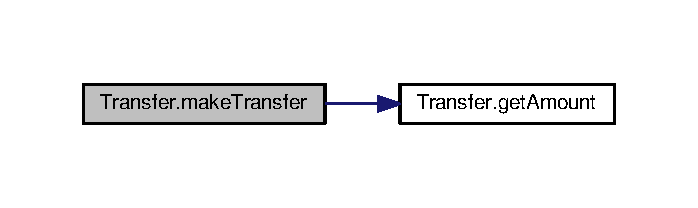
\includegraphics[width=335pt]{namespaceTransfer_a95da747b413b7cd0f8b22dfc81ab6a12_cgraph}
\end{center}
\end{figure}


\index{Transfer@{Transfer}!print\+Confirmation@{print\+Confirmation}}
\index{print\+Confirmation@{print\+Confirmation}!Transfer@{Transfer}}
\subsubsection[{\texorpdfstring{print\+Confirmation()}{printConfirmation()}}]{\setlength{\rightskip}{0pt plus 5cm}def Transfer.\+print\+Confirmation (
\begin{DoxyParamCaption}
{}
\end{DoxyParamCaption}
)}\hypertarget{namespaceTransfer_a71bccce92cfffa87bd8f8c1e90e9e5b6}{}\label{namespaceTransfer_a71bccce92cfffa87bd8f8c1e90e9e5b6}


Here is the call graph for this function\+:
\nopagebreak
\begin{figure}[H]
\begin{center}
\leavevmode
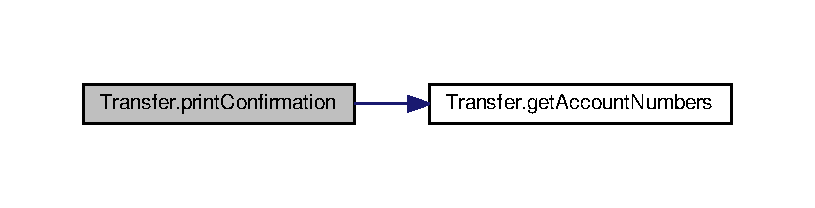
\includegraphics[width=350pt]{namespaceTransfer_a71bccce92cfffa87bd8f8c1e90e9e5b6_cgraph}
\end{center}
\end{figure}




\subsection{Variable Documentation}
\index{Transfer@{Transfer}!pin@{pin}}
\index{pin@{pin}!Transfer@{Transfer}}
\subsubsection[{\texorpdfstring{pin}{pin}}]{\setlength{\rightskip}{0pt plus 5cm}Transfer.\+pin = {\bf get\+P\+IN}(account\+One, account\+Two)}\hypertarget{namespaceTransfer_a623117f92f32121f4953c5a2622cfefa}{}\label{namespaceTransfer_a623117f92f32121f4953c5a2622cfefa}

\hypertarget{namespaceWelcome}{}\section{Welcome Namespace Reference}
\label{namespaceWelcome}\index{Welcome@{Welcome}}
\subsection*{Functions}
\begin{DoxyCompactItemize}
\item 
def \hyperlink{namespaceWelcome_ad84533550c8f8097042def3b70c84c5e}{get\+Username\+And\+Password} ()
\item 
def \hyperlink{namespaceWelcome_a613df5ce89bacc89b8666776ed895b7f}{retrieve\+Information} (u, p)
\item 
def \hyperlink{namespaceWelcome_a82b0eb139fe66dcdc216b43399db7069}{print\+Welcome} ()
\end{DoxyCompactItemize}


\subsection{Function Documentation}
\index{Welcome@{Welcome}!get\+Username\+And\+Password@{get\+Username\+And\+Password}}
\index{get\+Username\+And\+Password@{get\+Username\+And\+Password}!Welcome@{Welcome}}
\subsubsection[{\texorpdfstring{get\+Username\+And\+Password()}{getUsernameAndPassword()}}]{\setlength{\rightskip}{0pt plus 5cm}def Welcome.\+get\+Username\+And\+Password (
\begin{DoxyParamCaption}
{}
\end{DoxyParamCaption}
)}\hypertarget{namespaceWelcome_ad84533550c8f8097042def3b70c84c5e}{}\label{namespaceWelcome_ad84533550c8f8097042def3b70c84c5e}
\index{Welcome@{Welcome}!print\+Welcome@{print\+Welcome}}
\index{print\+Welcome@{print\+Welcome}!Welcome@{Welcome}}
\subsubsection[{\texorpdfstring{print\+Welcome()}{printWelcome()}}]{\setlength{\rightskip}{0pt plus 5cm}def Welcome.\+print\+Welcome (
\begin{DoxyParamCaption}
{}
\end{DoxyParamCaption}
)}\hypertarget{namespaceWelcome_a82b0eb139fe66dcdc216b43399db7069}{}\label{namespaceWelcome_a82b0eb139fe66dcdc216b43399db7069}


Here is the call graph for this function\+:
\nopagebreak
\begin{figure}[H]
\begin{center}
\leavevmode
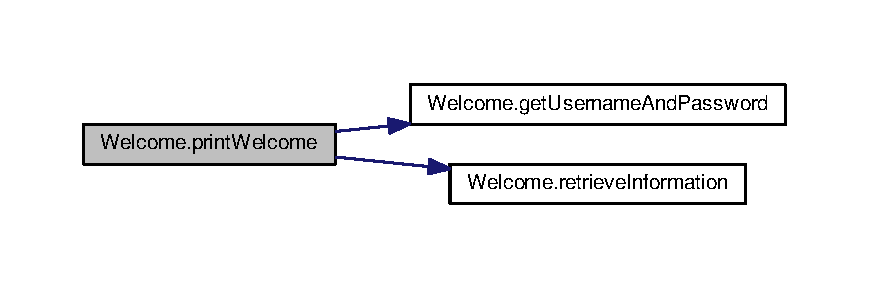
\includegraphics[width=350pt]{namespaceWelcome_a82b0eb139fe66dcdc216b43399db7069_cgraph}
\end{center}
\end{figure}


\index{Welcome@{Welcome}!retrieve\+Information@{retrieve\+Information}}
\index{retrieve\+Information@{retrieve\+Information}!Welcome@{Welcome}}
\subsubsection[{\texorpdfstring{retrieve\+Information(u, p)}{retrieveInformation(u, p)}}]{\setlength{\rightskip}{0pt plus 5cm}def Welcome.\+retrieve\+Information (
\begin{DoxyParamCaption}
\item[{}]{u, }
\item[{}]{p}
\end{DoxyParamCaption}
)}\hypertarget{namespaceWelcome_a613df5ce89bacc89b8666776ed895b7f}{}\label{namespaceWelcome_a613df5ce89bacc89b8666776ed895b7f}

\chapter{File Documentation}
\hypertarget{addAccount_8py}{}\section{add\+Account.\+py File Reference}
\label{addAccount_8py}\index{add\+Account.\+py@{add\+Account.\+py}}
\subsection*{Namespaces}
\begin{DoxyCompactItemize}
\item 
 \hyperlink{namespaceaddAccount}{add\+Account}
\end{DoxyCompactItemize}
\subsection*{Functions}
\begin{DoxyCompactItemize}
\item 
def \hyperlink{namespaceaddAccount_a3a8c94acd800e708964781259da98d47}{add\+Account.\+get\+Information} ()
\item 
def \hyperlink{namespaceaddAccount_ada25390ce86fe3bb69a36068bfb536e2}{add\+Account.\+create\+Account} (i, p)
\item 
def \hyperlink{namespaceaddAccount_adae774fe357f7b01357de9919b9e9da5}{add\+Account.\+set\+P\+IN} ()
\end{DoxyCompactItemize}
\subsection*{Variables}
\begin{DoxyCompactItemize}
\item 
\hyperlink{namespaceaddAccount_a54cf092e8aeaae1cd4b3d502f239ae08}{add\+Account.\+information} = get\+Information()
\item 
\hyperlink{namespaceaddAccount_ae10ea4b40c1517c05f038e86e63fb541}{add\+Account.\+pin} = set\+P\+IN()
\end{DoxyCompactItemize}

\hypertarget{Balance_8py}{}\section{Balance.\+py File Reference}
\label{Balance_8py}\index{Balance.\+py@{Balance.\+py}}
\subsection*{Namespaces}
\begin{DoxyCompactItemize}
\item 
 \hyperlink{namespaceBalance}{Balance}
\end{DoxyCompactItemize}
\subsection*{Functions}
\begin{DoxyCompactItemize}
\item 
def \hyperlink{namespaceBalance_a0d3d5e4b10843823c119cb200c8eea1a}{Balance.\+get\+Account\+Number} ()
\item 
def \hyperlink{namespaceBalance_add692cc47f5beab77cc3eded4397ee84}{Balance.\+get\+P\+IN} (n)
\item 
def \hyperlink{namespaceBalance_a2087471cfcf15c70932c7a400f6e8b00}{Balance.\+find\+Balance} (a, n)
\item 
def \hyperlink{namespaceBalance_afedee86fdf9a70c8269974c695523986}{Balance.\+print\+Balace} (b)
\end{DoxyCompactItemize}
\subsection*{Variables}
\begin{DoxyCompactItemize}
\item 
\hyperlink{namespaceBalance_a526eb4cc966158b4a4d3b8d33c04340f}{Balance.\+account\+Number} = get\+Account\+Number()
\item 
\hyperlink{namespaceBalance_a4cfe14f6e735fe18092e9809e4886137}{Balance.\+pin} = get\+P\+IN(account\+Number)
\item 
\hyperlink{namespaceBalance_a3a307687cae8694689c16220a9bb081c}{Balance.\+balance} = find\+Balance(account\+Number, pin)
\end{DoxyCompactItemize}

\hypertarget{Bank_8c}{}\section{Bank.\+c File Reference}
\label{Bank_8c}\index{Bank.\+c@{Bank.\+c}}
{\ttfamily \#include $<$stdio.\+h$>$}\\*
{\ttfamily \#include \char`\"{}/usr/include/python2.\+7/\+Python.\+h\char`\"{}}\\*
\subsection*{Functions}
\begin{DoxyCompactItemize}
\item 
void \hyperlink{Bank_8c_a355078f74f891a5fa3eefc513beba35a}{make\+Deposit} (int amount, F\+I\+LE $\ast$f)
\item 
void \hyperlink{Bank_8c_af4081bc28d6167f3de4d8df47e07b8b8}{check\+Balance} (int pin, F\+I\+LE $\ast$f)
\item 
void \hyperlink{Bank_8c_a32cb6019aee3f01c6aaf0560f3bba777}{transfer} (F\+I\+LE $\ast$f)
\item 
void \hyperlink{Bank_8c_ac08885164552631f8f0eae16e2330d73}{add\+New\+Account} (char type, F\+I\+LE $\ast$f)
\item 
int \hyperlink{Bank_8c_ae66f6b31b5ad750f1fe042a706a4e3d4}{main} ()
\end{DoxyCompactItemize}


\subsection{Function Documentation}
\index{Bank.\+c@{Bank.\+c}!add\+New\+Account@{add\+New\+Account}}
\index{add\+New\+Account@{add\+New\+Account}!Bank.\+c@{Bank.\+c}}
\subsubsection[{\texorpdfstring{add\+New\+Account(char type, F\+I\+L\+E $\ast$f)}{addNewAccount(char type, FILE *f)}}]{\setlength{\rightskip}{0pt plus 5cm}void add\+New\+Account (
\begin{DoxyParamCaption}
\item[{char}]{type, }
\item[{F\+I\+LE $\ast$}]{f}
\end{DoxyParamCaption}
)}\hypertarget{Bank_8c_ac08885164552631f8f0eae16e2330d73}{}\label{Bank_8c_ac08885164552631f8f0eae16e2330d73}
\index{Bank.\+c@{Bank.\+c}!check\+Balance@{check\+Balance}}
\index{check\+Balance@{check\+Balance}!Bank.\+c@{Bank.\+c}}
\subsubsection[{\texorpdfstring{check\+Balance(int pin, F\+I\+L\+E $\ast$f)}{checkBalance(int pin, FILE *f)}}]{\setlength{\rightskip}{0pt plus 5cm}void check\+Balance (
\begin{DoxyParamCaption}
\item[{int}]{pin, }
\item[{F\+I\+LE $\ast$}]{f}
\end{DoxyParamCaption}
)}\hypertarget{Bank_8c_af4081bc28d6167f3de4d8df47e07b8b8}{}\label{Bank_8c_af4081bc28d6167f3de4d8df47e07b8b8}
\index{Bank.\+c@{Bank.\+c}!main@{main}}
\index{main@{main}!Bank.\+c@{Bank.\+c}}
\subsubsection[{\texorpdfstring{main()}{main()}}]{\setlength{\rightskip}{0pt plus 5cm}int main (
\begin{DoxyParamCaption}
{}
\end{DoxyParamCaption}
)}\hypertarget{Bank_8c_ae66f6b31b5ad750f1fe042a706a4e3d4}{}\label{Bank_8c_ae66f6b31b5ad750f1fe042a706a4e3d4}


Here is the call graph for this function\+:
\nopagebreak
\begin{figure}[H]
\begin{center}
\leavevmode
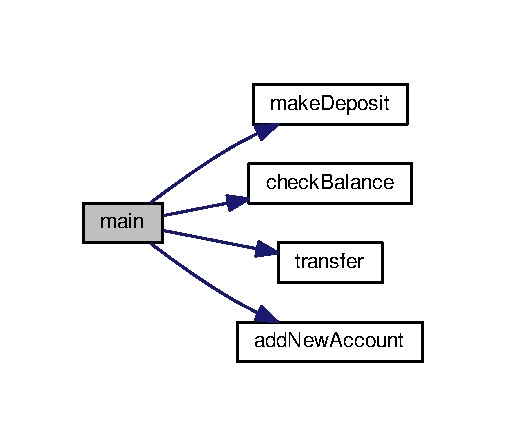
\includegraphics[width=243pt]{Bank_8c_ae66f6b31b5ad750f1fe042a706a4e3d4_cgraph}
\end{center}
\end{figure}


\index{Bank.\+c@{Bank.\+c}!make\+Deposit@{make\+Deposit}}
\index{make\+Deposit@{make\+Deposit}!Bank.\+c@{Bank.\+c}}
\subsubsection[{\texorpdfstring{make\+Deposit(int amount, F\+I\+L\+E $\ast$f)}{makeDeposit(int amount, FILE *f)}}]{\setlength{\rightskip}{0pt plus 5cm}void make\+Deposit (
\begin{DoxyParamCaption}
\item[{int}]{amount, }
\item[{F\+I\+LE $\ast$}]{f}
\end{DoxyParamCaption}
)}\hypertarget{Bank_8c_a355078f74f891a5fa3eefc513beba35a}{}\label{Bank_8c_a355078f74f891a5fa3eefc513beba35a}
\index{Bank.\+c@{Bank.\+c}!transfer@{transfer}}
\index{transfer@{transfer}!Bank.\+c@{Bank.\+c}}
\subsubsection[{\texorpdfstring{transfer(\+F\+I\+L\+E $\ast$f)}{transfer(FILE *f)}}]{\setlength{\rightskip}{0pt plus 5cm}void transfer (
\begin{DoxyParamCaption}
\item[{F\+I\+LE $\ast$}]{f}
\end{DoxyParamCaption}
)}\hypertarget{Bank_8c_a32cb6019aee3f01c6aaf0560f3bba777}{}\label{Bank_8c_a32cb6019aee3f01c6aaf0560f3bba777}

\hypertarget{Bank_8c__ast_8txt}{}\section{Bank.\+c\+\_\+ast.\+txt File Reference}
\label{Bank_8c__ast_8txt}\index{Bank.\+c\+\_\+ast.\+txt@{Bank.\+c\+\_\+ast.\+txt}}

\hypertarget{Bank_8c__ast__OG_8txt}{}\section{Bank.\+c\+\_\+ast\+\_\+\+O\+G.\+txt File Reference}
\label{Bank_8c__ast__OG_8txt}\index{Bank.\+c\+\_\+ast\+\_\+\+O\+G.\+txt@{Bank.\+c\+\_\+ast\+\_\+\+O\+G.\+txt}}

\hypertarget{Deposit_8py}{}\section{Deposit.\+py File Reference}
\label{Deposit_8py}\index{Deposit.\+py@{Deposit.\+py}}
\subsection*{Namespaces}
\begin{DoxyCompactItemize}
\item 
 \hyperlink{namespaceDeposit}{Deposit}
\end{DoxyCompactItemize}
\subsection*{Functions}
\begin{DoxyCompactItemize}
\item 
def \hyperlink{namespaceDeposit_a5550db47d340cfbf8da0504fdbb4bd38}{Deposit.\+get\+Account\+Number} ()
\item 
def \hyperlink{namespaceDeposit_aeb2bde95c577d37691610d458bba8d96}{Deposit.\+get\+P\+IN} (n)
\item 
def \hyperlink{namespaceDeposit_a1980b46e5ca4ad7fe16e06703b568f78}{Deposit.\+get\+Amount} ()
\item 
def \hyperlink{namespaceDeposit_ae5cbbb64bef92d28ac3283006f0ac72c}{Deposit.\+take\+Picture\+Of\+Check} ()
\item 
def \hyperlink{namespaceDeposit_ae9c9febfed3a8d6ad618d2c123df4b77}{Deposit.\+deposit\+Check} (n, p, a)
\item 
def \hyperlink{namespaceDeposit_a7d4afe0289e672f39e4951c790cf8927}{Deposit.\+print\+Confirmation} ()
\end{DoxyCompactItemize}
\subsection*{Variables}
\begin{DoxyCompactItemize}
\item 
\hyperlink{namespaceDeposit_a266a490bcb8b7e116e4e7258429aabe5}{Deposit.\+account\+Number} = get\+Account\+Number()
\item 
\hyperlink{namespaceDeposit_a5ae26ec6c68e4031fbb50c9b0b15daf7}{Deposit.\+pin} = get\+P\+IN()
\item 
\hyperlink{namespaceDeposit_a903d2b091ff78ff14bb2e0e6b002de77}{Deposit.\+amount} = get\+Amount()
\end{DoxyCompactItemize}

\hypertarget{ex1_8c}{}\section{ex1.\+c File Reference}
\label{ex1_8c}\index{ex1.\+c@{ex1.\+c}}
{\ttfamily \#include $<$python2.\+7/\+Python.\+h$>$}\\*
{\ttfamily \#include $<$stdio.\+h$>$}\\*
Include dependency graph for ex1.\+c\+:
\nopagebreak
\begin{figure}[H]
\begin{center}
\leavevmode
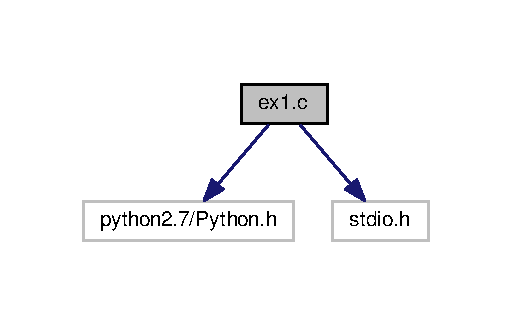
\includegraphics[width=246pt]{ex1_8c__incl}
\end{center}
\end{figure}
\subsection*{Functions}
\begin{DoxyCompactItemize}
\item 
int \hyperlink{ex1_8c_ae66f6b31b5ad750f1fe042a706a4e3d4}{main} ()
\end{DoxyCompactItemize}


\subsection{Function Documentation}
\index{ex1.\+c@{ex1.\+c}!main@{main}}
\index{main@{main}!ex1.\+c@{ex1.\+c}}
\subsubsection[{\texorpdfstring{main()}{main()}}]{\setlength{\rightskip}{0pt plus 5cm}int main (
\begin{DoxyParamCaption}
{}
\end{DoxyParamCaption}
)}\hypertarget{ex1_8c_ae66f6b31b5ad750f1fe042a706a4e3d4}{}\label{ex1_8c_ae66f6b31b5ad750f1fe042a706a4e3d4}

\hypertarget{ex1_8c__ast_8txt}{}\section{ex1.\+c\+\_\+ast.\+txt File Reference}
\label{ex1_8c__ast_8txt}\index{ex1.\+c\+\_\+ast.\+txt@{ex1.\+c\+\_\+ast.\+txt}}

\hypertarget{ex1_8c__ast__OG_8txt}{}\section{ex1.\+c\+\_\+ast\+\_\+\+O\+G.\+txt File Reference}
\label{ex1_8c__ast__OG_8txt}\index{ex1.\+c\+\_\+ast\+\_\+\+O\+G.\+txt@{ex1.\+c\+\_\+ast\+\_\+\+O\+G.\+txt}}

\hypertarget{ex1_8py}{}\section{ex1.\+py File Reference}
\label{ex1_8py}\index{ex1.\+py@{ex1.\+py}}
\subsection*{Namespaces}
\begin{DoxyCompactItemize}
\item 
 \hyperlink{namespaceex1}{ex1}
\end{DoxyCompactItemize}
\subsection*{Functions}
\begin{DoxyCompactItemize}
\item 
def \hyperlink{namespaceex1_ad41019fd953cd7d2a406a9f2fb674128}{ex1.\+hello} (a, b)
\end{DoxyCompactItemize}

\hypertarget{ex2_8c}{}\section{ex2.\+c File Reference}
\label{ex2_8c}\index{ex2.\+c@{ex2.\+c}}
{\ttfamily \#include \char`\"{}stdio.\+h\char`\"{}}\\*
{\ttfamily \#include $<$python2.\+7/\+Python.\+h$>$}\\*
Include dependency graph for ex2.\+c\+:
\nopagebreak
\begin{figure}[H]
\begin{center}
\leavevmode
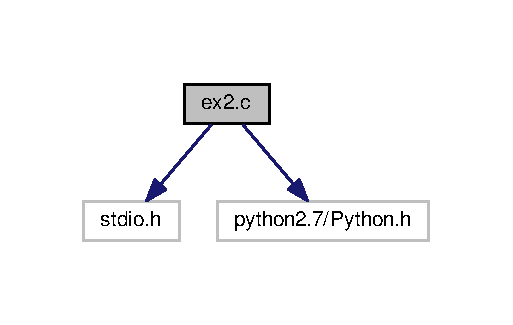
\includegraphics[width=246pt]{ex2_8c__incl}
\end{center}
\end{figure}
\subsection*{Functions}
\begin{DoxyCompactItemize}
\item 
int \hyperlink{ex2_8c_a9ef43c94a04d3145f5f315231da4526e}{main} (int argc, \+\_\+\+T\+C\+H\+AR $\ast$argv\mbox{[}$\,$\mbox{]})
\end{DoxyCompactItemize}


\subsection{Function Documentation}
\index{ex2.\+c@{ex2.\+c}!main@{main}}
\index{main@{main}!ex2.\+c@{ex2.\+c}}
\subsubsection[{\texorpdfstring{main(int argc, \+\_\+\+T\+C\+H\+A\+R $\ast$argv[])}{main(int argc, _TCHAR *argv[])}}]{\setlength{\rightskip}{0pt plus 5cm}int main (
\begin{DoxyParamCaption}
\item[{int}]{argc, }
\item[{\+\_\+\+T\+C\+H\+AR $\ast$}]{argv\mbox{[}$\,$\mbox{]}}
\end{DoxyParamCaption}
)}\hypertarget{ex2_8c_a9ef43c94a04d3145f5f315231da4526e}{}\label{ex2_8c_a9ef43c94a04d3145f5f315231da4526e}

\hypertarget{ex2_8c__ast_8txt}{}\section{ex2.\+c\+\_\+ast.\+txt File Reference}
\label{ex2_8c__ast_8txt}\index{ex2.\+c\+\_\+ast.\+txt@{ex2.\+c\+\_\+ast.\+txt}}

\hypertarget{ex2_8c__ast__OG_8txt}{}\section{ex2.\+c\+\_\+ast\+\_\+\+O\+G.\+txt File Reference}
\label{ex2_8c__ast__OG_8txt}\index{ex2.\+c\+\_\+ast\+\_\+\+O\+G.\+txt@{ex2.\+c\+\_\+ast\+\_\+\+O\+G.\+txt}}

\hypertarget{ex2_8py}{}\section{ex2.\+py File Reference}
\label{ex2_8py}\index{ex2.\+py@{ex2.\+py}}
\subsection*{Namespaces}
\begin{DoxyCompactItemize}
\item 
 \hyperlink{namespaceex2}{ex2}
\end{DoxyCompactItemize}
\subsection*{Functions}
\begin{DoxyCompactItemize}
\item 
def \hyperlink{namespaceex2_a9a47f35041ae3cec88184ca43faaabc1}{ex2.\+func1} (a, b)
\end{DoxyCompactItemize}

\hypertarget{ex3_8cpp}{}\section{ex3.\+cpp File Reference}
\label{ex3_8cpp}\index{ex3.\+cpp@{ex3.\+cpp}}
{\ttfamily \#include $<$iostream$>$}\\*
{\ttfamily \#include $<$python2.\+7/\+Python.\+h$>$}\\*
Include dependency graph for ex3.\+cpp\+:
\nopagebreak
\begin{figure}[H]
\begin{center}
\leavevmode
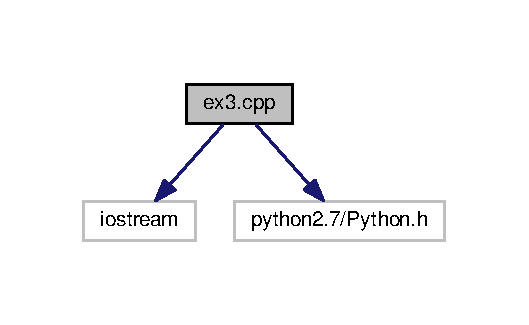
\includegraphics[width=254pt]{ex3_8cpp__incl}
\end{center}
\end{figure}
\subsection*{Functions}
\begin{DoxyCompactItemize}
\item 
int \hyperlink{ex3_8cpp_ae66f6b31b5ad750f1fe042a706a4e3d4}{main} ()
\end{DoxyCompactItemize}


\subsection{Function Documentation}
\index{ex3.\+cpp@{ex3.\+cpp}!main@{main}}
\index{main@{main}!ex3.\+cpp@{ex3.\+cpp}}
\subsubsection[{\texorpdfstring{main()}{main()}}]{\setlength{\rightskip}{0pt plus 5cm}int main (
\begin{DoxyParamCaption}
{}
\end{DoxyParamCaption}
)}\hypertarget{ex3_8cpp_ae66f6b31b5ad750f1fe042a706a4e3d4}{}\label{ex3_8cpp_ae66f6b31b5ad750f1fe042a706a4e3d4}

\hypertarget{ex3_8cpp__ast_8txt}{}\section{ex3.\+cpp\+\_\+ast.\+txt File Reference}
\label{ex3_8cpp__ast_8txt}\index{ex3.\+cpp\+\_\+ast.\+txt@{ex3.\+cpp\+\_\+ast.\+txt}}

\hypertarget{ex3_8cpp__ast__OG_8txt}{}\section{ex3.\+cpp\+\_\+ast\+\_\+\+O\+G.\+txt File Reference}
\label{ex3_8cpp__ast__OG_8txt}\index{ex3.\+cpp\+\_\+ast\+\_\+\+O\+G.\+txt@{ex3.\+cpp\+\_\+ast\+\_\+\+O\+G.\+txt}}

\hypertarget{ex3_8py}{}\section{ex3.\+py File Reference}
\label{ex3_8py}\index{ex3.\+py@{ex3.\+py}}
\subsection*{Namespaces}
\begin{DoxyCompactItemize}
\item 
 \hyperlink{namespaceex3}{ex3}
\end{DoxyCompactItemize}

\hypertarget{ex4_8c}{}\section{ex4.\+c File Reference}
\label{ex4_8c}\index{ex4.\+c@{ex4.\+c}}
{\ttfamily \#include $<$python2.\+7/\+Python.\+h$>$}\\*
Include dependency graph for ex4.\+c\+:
\nopagebreak
\begin{figure}[H]
\begin{center}
\leavevmode
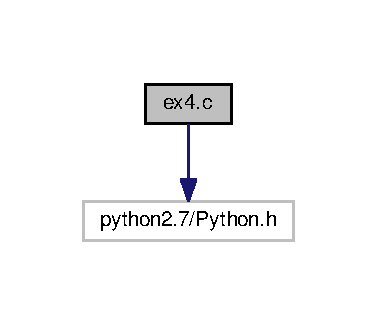
\includegraphics[width=181pt]{ex4_8c__incl}
\end{center}
\end{figure}
\subsection*{Macros}
\begin{DoxyCompactItemize}
\item 
\#define \hyperlink{ex4_8c_a2a3ad4ebb43e29f804a1e524aca840b2}{I\+N\+P\+U\+T\+\_\+\+F\+I\+LE}~\char`\"{}ex4.\+py\char`\"{}
\end{DoxyCompactItemize}
\subsection*{Functions}
\begin{DoxyCompactItemize}
\item 
int \hyperlink{ex4_8c_ae66f6b31b5ad750f1fe042a706a4e3d4}{main} ()
\end{DoxyCompactItemize}


\subsection{Macro Definition Documentation}
\index{ex4.\+c@{ex4.\+c}!I\+N\+P\+U\+T\+\_\+\+F\+I\+LE@{I\+N\+P\+U\+T\+\_\+\+F\+I\+LE}}
\index{I\+N\+P\+U\+T\+\_\+\+F\+I\+LE@{I\+N\+P\+U\+T\+\_\+\+F\+I\+LE}!ex4.\+c@{ex4.\+c}}
\subsubsection[{\texorpdfstring{I\+N\+P\+U\+T\+\_\+\+F\+I\+LE}{INPUT_FILE}}]{\setlength{\rightskip}{0pt plus 5cm}\#define I\+N\+P\+U\+T\+\_\+\+F\+I\+LE~\char`\"{}ex4.\+py\char`\"{}}\hypertarget{ex4_8c_a2a3ad4ebb43e29f804a1e524aca840b2}{}\label{ex4_8c_a2a3ad4ebb43e29f804a1e524aca840b2}


\subsection{Function Documentation}
\index{ex4.\+c@{ex4.\+c}!main@{main}}
\index{main@{main}!ex4.\+c@{ex4.\+c}}
\subsubsection[{\texorpdfstring{main()}{main()}}]{\setlength{\rightskip}{0pt plus 5cm}int main (
\begin{DoxyParamCaption}
{}
\end{DoxyParamCaption}
)}\hypertarget{ex4_8c_ae66f6b31b5ad750f1fe042a706a4e3d4}{}\label{ex4_8c_ae66f6b31b5ad750f1fe042a706a4e3d4}

\hypertarget{ex4_8c__ast_8txt}{}\section{ex4.\+c\+\_\+ast.\+txt File Reference}
\label{ex4_8c__ast_8txt}\index{ex4.\+c\+\_\+ast.\+txt@{ex4.\+c\+\_\+ast.\+txt}}

\hypertarget{ex4_8c__ast__OG_8txt}{}\section{ex4.\+c\+\_\+ast\+\_\+\+O\+G.\+txt File Reference}
\label{ex4_8c__ast__OG_8txt}\index{ex4.\+c\+\_\+ast\+\_\+\+O\+G.\+txt@{ex4.\+c\+\_\+ast\+\_\+\+O\+G.\+txt}}

\hypertarget{ex4_8py}{}\section{ex4.\+py File Reference}
\label{ex4_8py}\index{ex4.\+py@{ex4.\+py}}
\subsection*{Namespaces}
\begin{DoxyCompactItemize}
\item 
 \hyperlink{namespaceex4}{ex4}
\end{DoxyCompactItemize}

\hypertarget{ex5_8c}{}\section{ex5.\+c File Reference}
\label{ex5_8c}\index{ex5.\+c@{ex5.\+c}}
{\ttfamily \#include $<$stdio.\+h$>$}\\*
{\ttfamily \#include $<$python2.\+7/\+Python.\+h$>$}\\*
Include dependency graph for ex5.\+c\+:
\nopagebreak
\begin{figure}[H]
\begin{center}
\leavevmode
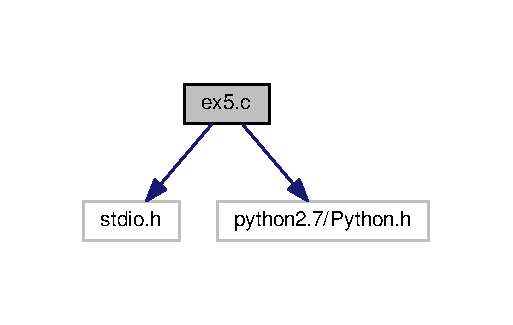
\includegraphics[width=246pt]{ex5_8c__incl}
\end{center}
\end{figure}
\subsection*{Functions}
\begin{DoxyCompactItemize}
\item 
int \hyperlink{ex5_8c_a0ddf1224851353fc92bfbff6f499fa97}{main} (int argc, char $\ast$argv\mbox{[}$\,$\mbox{]})
\end{DoxyCompactItemize}


\subsection{Function Documentation}
\index{ex5.\+c@{ex5.\+c}!main@{main}}
\index{main@{main}!ex5.\+c@{ex5.\+c}}
\subsubsection[{\texorpdfstring{main(int argc, char $\ast$argv[])}{main(int argc, char *argv[])}}]{\setlength{\rightskip}{0pt plus 5cm}int main (
\begin{DoxyParamCaption}
\item[{int}]{argc, }
\item[{char $\ast$}]{argv\mbox{[}$\,$\mbox{]}}
\end{DoxyParamCaption}
)}\hypertarget{ex5_8c_a0ddf1224851353fc92bfbff6f499fa97}{}\label{ex5_8c_a0ddf1224851353fc92bfbff6f499fa97}

\hypertarget{ex5_8c__ast_8txt}{}\section{ex5.\+c\+\_\+ast.\+txt File Reference}
\label{ex5_8c__ast_8txt}\index{ex5.\+c\+\_\+ast.\+txt@{ex5.\+c\+\_\+ast.\+txt}}

\hypertarget{ex5_8c__ast__OG_8txt}{}\section{ex5.\+c\+\_\+ast\+\_\+\+O\+G.\+txt File Reference}
\label{ex5_8c__ast__OG_8txt}\index{ex5.\+c\+\_\+ast\+\_\+\+O\+G.\+txt@{ex5.\+c\+\_\+ast\+\_\+\+O\+G.\+txt}}

\hypertarget{ex5_8py}{}\section{ex5.\+py File Reference}
\label{ex5_8py}\index{ex5.\+py@{ex5.\+py}}
\subsection*{Namespaces}
\begin{DoxyCompactItemize}
\item 
 \hyperlink{namespaceex5}{ex5}
\end{DoxyCompactItemize}

\hypertarget{Transfer_8py}{}\section{Transfer.\+py File Reference}
\label{Transfer_8py}\index{Transfer.\+py@{Transfer.\+py}}
\subsection*{Namespaces}
\begin{DoxyCompactItemize}
\item 
 \hyperlink{namespaceTransfer}{Transfer}
\end{DoxyCompactItemize}
\subsection*{Functions}
\begin{DoxyCompactItemize}
\item 
def \hyperlink{namespaceTransfer_a16590530b35d7e0d18fbb42ab67f4ef3}{Transfer.\+get\+Account\+Numbers} ()
\item 
def \hyperlink{namespaceTransfer_a0c1b371151be67118901e82b8187b2c3}{Transfer.\+get\+P\+IN} (a, b)
\item 
def \hyperlink{namespaceTransfer_a11908eef096879f9b9a7ca569ba079aa}{Transfer.\+get\+Amount} ()
\item 
def \hyperlink{namespaceTransfer_a95da747b413b7cd0f8b22dfc81ab6a12}{Transfer.\+make\+Transfer} (a, b, p)
\item 
def \hyperlink{namespaceTransfer_a71bccce92cfffa87bd8f8c1e90e9e5b6}{Transfer.\+print\+Confirmation} ()
\end{DoxyCompactItemize}
\subsection*{Variables}
\begin{DoxyCompactItemize}
\item 
\hyperlink{namespaceTransfer_a623117f92f32121f4953c5a2622cfefa}{Transfer.\+pin} = get\+P\+IN(account\+One, account\+Two)
\end{DoxyCompactItemize}

\hypertarget{Welcome_8py}{}\section{Welcome.\+py File Reference}
\label{Welcome_8py}\index{Welcome.\+py@{Welcome.\+py}}
\subsection*{Namespaces}
\begin{DoxyCompactItemize}
\item 
 \hyperlink{namespaceWelcome}{Welcome}
\end{DoxyCompactItemize}
\subsection*{Functions}
\begin{DoxyCompactItemize}
\item 
def \hyperlink{namespaceWelcome_ad84533550c8f8097042def3b70c84c5e}{Welcome.\+get\+Username\+And\+Password} ()
\item 
def \hyperlink{namespaceWelcome_a613df5ce89bacc89b8666776ed895b7f}{Welcome.\+retrieve\+Information} (u, p)
\item 
def \hyperlink{namespaceWelcome_a82b0eb139fe66dcdc216b43399db7069}{Welcome.\+print\+Welcome} ()
\end{DoxyCompactItemize}

%--- End generated contents ---

% Index
\backmatter
\newpage
\phantomsection
\clearemptydoublepage
\addcontentsline{toc}{chapter}{Index}
\printindex

\end{document}
